\documentclass{article}
\usepackage{amsmath}
\usepackage{xcolor}
\usepackage{gensymb}
\usepackage{ragged2e}
\usepackage{graphicx}
\usepackage{gensymb}
\usepackage{mathtools}
\usepackage{amssymb}
\newcommand{\mydet}[1]{\ensuremath{\begin{vmatrix}#1\end{vmatrix}}}
\providecommand{\brak}[1]{\ensuremath{\left(#1\right)}}
\providecommand{\norm}[1]{\left\lVert#1\right\rVert}
\newcommand{\solution}{\noindent \textbf{Solution: }}
\newcommand{\myvec}[1]{\ensuremath{\begin{pmatrix}#1\end{pmatrix}}}
\let\vec\mathbf
\begin{document}
\begin{center}
        \textbf\large{CHAPTER-9 \\ TRIANGLES}
\end{center}
\section{Exercise 9.2}
Q4. $\vec{P}$ is a point in the interior of a parallelogram $ABCD$.Show that
\begin{enumerate} 
\item $ar(APB)+Ar(PCD) = \frac{1}{2}ar(ABCD)$
\item $ar(APD)+ar(PBC) = ar(APB)+ar(PCD)$   
\end{enumerate}	

\begin{table}[h]
	  \centering
	  
\begin{tabular}{|c|c|c|}
\hline
Components & Value & Quantity\\
\hline
Resistor & 220 Ohm & 1\\
\hline
Arduino & UNO & 1\\
\hline
Bread Board & & 1\\
\hline
Jumper Wires & M-M & 10\\
\hline
LED & & 1\\
\hline
\end{tabular}

	  \caption{Parameters}
	  \label{tab:Table1}
\end{table}

\section{Solution}
As the area of a parallelogram with adjacent sides $a$ and $b$ is,
\begin{align}
\text{Area of parallelogram = } \norm{\vec{a} \times \vec{b}}
\label{eq-1-}
\end{align}
And, area of a triangle with adjacent sides $p$ and $q$ is,
\begin{align}
\text{Area of triangle = } \frac{1}{2} \norm{\vec{p} \times \vec{q}}
\label{eq-2-}
\end{align}
So,
\begin{align}
\norm{\vec{A-D}} = \norm{\vec{B-C}}
\label{eq-3-}
\end{align}
Consider $\triangle APD$
\begin{align}
Ar(APD) = \frac{1}{2}\norm{\vec{(A-D)} \times \vec{(A-P)}}
\label{eq-4-}
\end{align}
Consider $\triangle PBC$
\begin{align}
Ar(BPC) =  \frac{1}{2}\norm{\vec{(B-C)} \times \vec{(P-B)}}
\label{eq-5-}
\end{align}
On adding \eqref{eq-4-} and \eqref{eq-5-},
\begin{multline}
Ar(APD) + Ar(PBC) =\\
 \frac{1}{2}\norm{\vec{(A-D)} \times \vec{(A-P)}} + \frac{1}{2}\norm{\vec{(B-C)} \times \vec{(P-B)}}
\label{eq-6-}
\end{multline}
From equation \eqref{eq-3-},
\begin{multline}
Ar(APD) + Ar(PBC) =\\
 \frac{1}{2}\norm{\vec{(A-D)} \times \vec{(A-P)}} + \frac{1}{2}\norm{\vec{(A-D)} \times \vec{(P-B)}}
\label{eq-7-}
\end{multline}
\begin{multline}
\implies Ar(APD) + Ar(PBC) =\\ \frac{1}{2}\norm{\vec{(A-D)}\times[\vec{(A-P)} + \vec{(P-B)}]}
\label{eq-8-}
\end{multline}
Here, $AP$ and $PB$ are adjacent sides of $\triangle$ $APB$
\\From Triangle law of vector addition, \\ $\vec{(A-P)} + \vec{(P-B)} = \vec{(A-B)}$
\begin{align}
\implies Ar(APD) + Ar(PBC) = \frac{1}{2}\norm{\vec{(A-D)}\times\vec{(A-B)}}
\label{eq-9-}
\end{align}
Since, $\vec{(A-D)} \text{ and }\vec{(A-B)}$ are adjacent sides of paralleogram ABCD
\\From \eqref{eq-2-},
\begin{align}
Ar(ABCD) = \norm{\vec{(A-D)}\times\vec{(A-B)}}
\label{eq-10-}
\end{align}
From \eqref{eq-9-} and \eqref{eq-10-}
\begin{align}
\therefore  Ar(APD)+Ar(PBC) = \frac{1}{2}Ar(ABCD)
\label{eq-11-}
\end{align}


Similarly, we can prove that,
\begin{align}
Ar(APB)+Ar(PBD) = \frac{1}{2}Ar(ABCD)
\label{eq-12-}
\end{align}
On Comparing \eqref{eq-11-} and \eqref{eq-12-},
\begin{align}
Ar(APD)+Ar(PBC) = Ar(APB)+Ar(PCD)
\label{eq-13-}
\end{align}

\begin{figure}[!ht]
	\begin{center}
		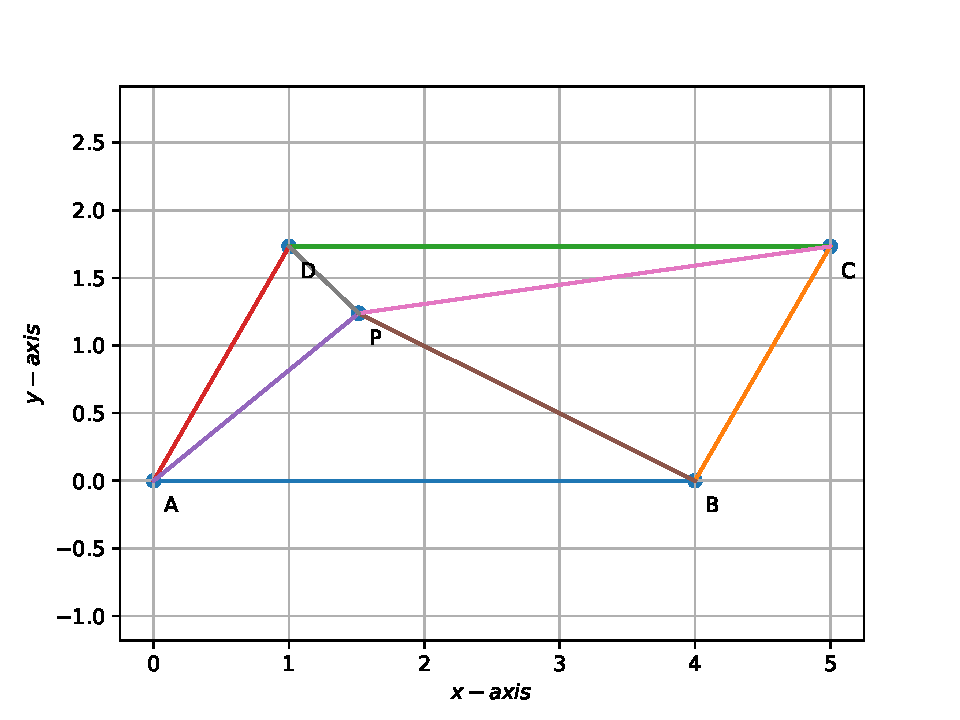
\includegraphics[width=\columnwidth]{figs/fig.pdf}
	\end{center}
	\caption{Parallelogram ABCD with interior point P}
\label{fig:Parallelogram}
\end{figure}
\end{document}
